\documentclass[notes,slidesec,a4]{seminar}

\usepackage[utf8]{inputenc}
\usepackage[spanish]{babel} % espanol


\usepackage{t-gsyc-6}
\usepackage{fancybox}
\usepackage{graphics}
\usepackage{moreverb}
\usepackage{alltt}
\usepackage{html}
\usepackage{color}
\usepackage[usenames,dvipsnames,svgnames,table]{xcolor}
\usepackage{amsmath}
\usepackage[normalsize]{subfigure}
\usepackage{url}
\usepackage{hyperref}
\usepackage{listings}
\usepackage{multirow}


\title{MANEJO DE UN DRONE CON
%\\ \vspace{0.2cm} 
 WEBRTC Y JDEROBOT}
\author{Iván Rodríguez-Bobada Martín}

\cop{Iván Rodríguez-Bobada Martín}
\address{i.rodriguezmar@alumnos.urjc.es}

\begin{document}
\maketitle

%%--------------------------------------------------------------

\begin{hslide}
\slsect{Índice}
\begin{itemize}
\item Introducción 
\item Objetivos
\item Infraestructura
\item Desarrollo software
\item Experimentos
\item Conclusiones
\end{itemize}
\end{hslide}


%%--------------------------------------------------------------

\begin{hslide}
\slsect{Introducción}
\slsubsect{Aplicaciones de los drones}
\begin{minipage}[t]{0.5\textwidth}
\begin{center}
\begin{figure}
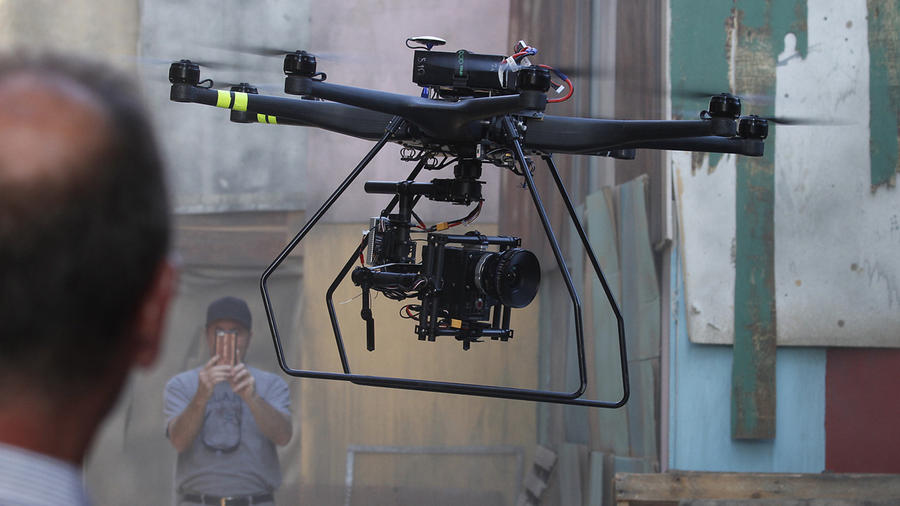
\includegraphics[width=0.7\textwidth]{img/dronefilm}
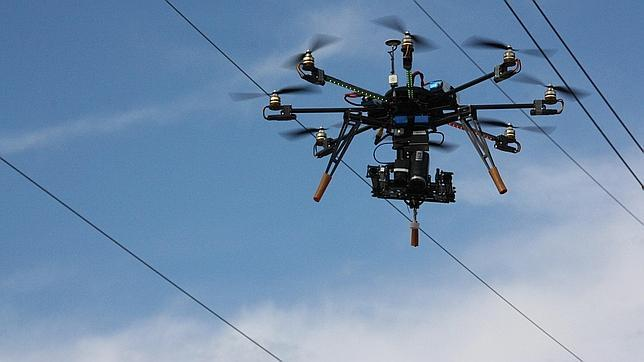
\includegraphics[width=0.7\textwidth]{img/dronendesa}
\end{figure}
\end{center}
\end{minipage}
\begin{minipage}[t]{0.5\textwidth}
\begin{center}
\begin{figure}
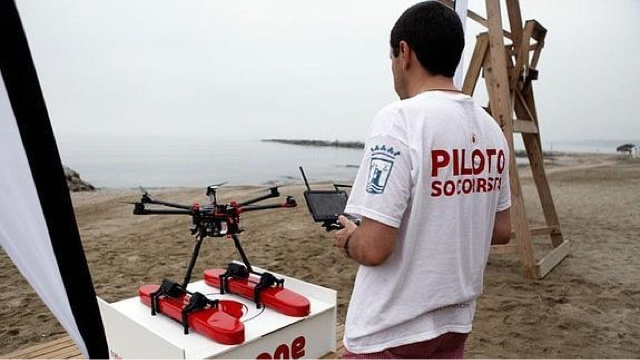
\includegraphics[width=0.7\textwidth]{img/socorrista}
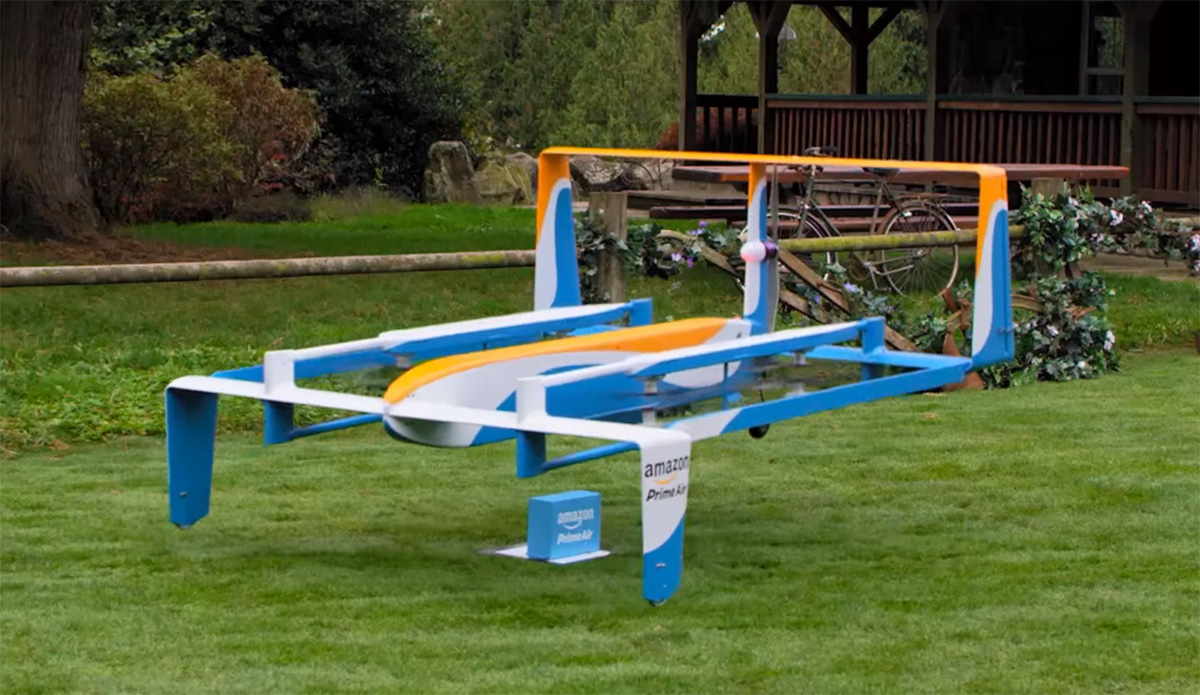
\includegraphics[width=0.7\textwidth]{img/amazon}
\end{figure}
\end{center}
\end{minipage}
\end{hslide}

%%--------------------------------------------------------------


\begin{hslide}
\slsubsect{Antecedentes: Surveillance 5.1}
\begin{itemize}
\item TFG de Edgar Barrero.
\item Desarrollado con Ruby on Rails.
\item Un servidor web intermedio se conecta a los servidores ICE.
\end{itemize}
\begin{minipage}[t]{0.3\textwidth}
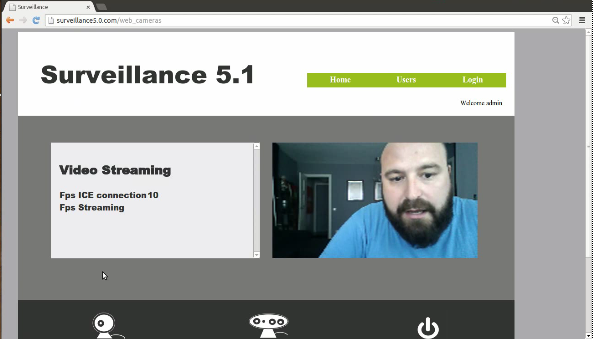
\includegraphics[width=\textwidth]{img/surveillance5}
\end{minipage}
\begin{minipage}[t]{0.7\textwidth}
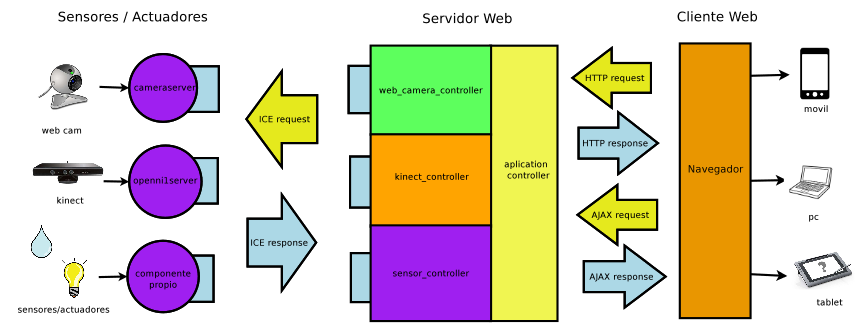
\includegraphics[width=\textwidth]{img/esquema_s5}
\end{minipage}
\end{hslide}


%%--------------------------------------------------------------


\begin{hslide}
\slsubsect{Antecedentes: Teleoperadores y visores Web en JdeRobot}
\begin{itemize}
\item TFG de Aitor Martínez.
\item Desarrollado directamente en el navegador con JavaScript.
\item Conexión con sensores y actuadores sin servidores intermedios.
\end{itemize}
\begin{center}
\begin{figure}
\includegraphics[width=0.7\textwidth]{img/uavviewerjs_aitor}
\end{figure}
\end{center}
\end{hslide}

%%--------------------------------------------------------------

\begin{hslide}
\slsect{Objetivo}
Teleoperar un drone con tecnologías web de última generación (WebRTC)
sin servidores intermedios desde multidispositivos.

Sub-objetivos:
\begin{itemize}
\item Conexión local: par local - drone.
\item Conexión remota entre pares: par local - par remoto.
\item Interfaz web de usuario amigable e intuitiva.
\end{itemize}
\end{hslide}

%%--------------------------------------------------------------

\begin{hslide}
\slsect{Infraestructura}
\begin{minipage}[t]{0.7\textwidth}
\begin{itemize}
\item ArDrone2.0 de Parrot
\item Simulador Gazebo
\item ICE: \emph{Middleware} para conexiones
\item JdeRobot:
\begin{itemize}
\item \emph{Plugin de Gazebo}: Versión virtual del drone.
\item \emph{ArDroneServer}: Servidor del drone real.
\end{itemize}
\end{itemize}
\end{minipage}
\begin{minipage}[t]{0.3\textwidth}
\begin{center}
\begin{figure}
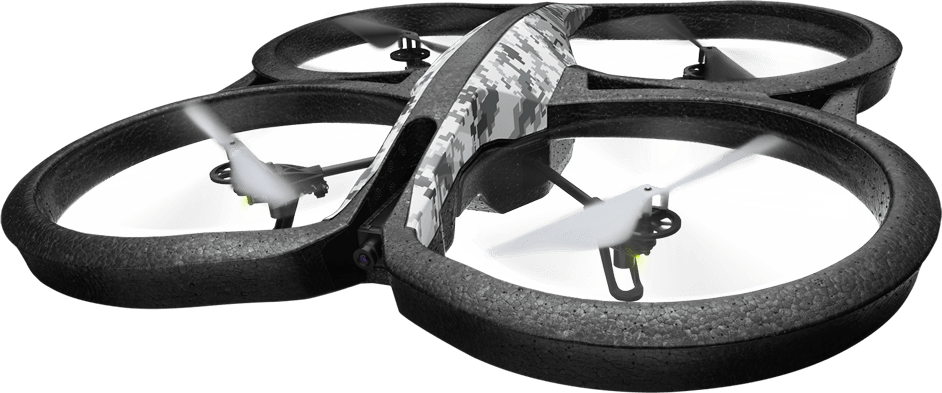
\includegraphics[width=0.8\textwidth]{img/ardrone}
\end{figure}
\end{center}
\begin{center}
\begin{figure}

\includegraphics[width=0.8\textwidth]{img/jderobot}
\end{figure}
\end{center}
\end{minipage}
\end{hslide}




%%--------------------------------------------------------------


\begin{hslide}
\slsubsect{WebRTC}
\begin{itemize}
\item Tecnología de comunicaciones entre navegadores en tiempo real.
\item Transmisión de audio, vídeo y datos.
\item Sin necesidad de servidores intermedios.
\end{itemize}
\begin{center}
\begin{figure}

\includegraphics[width=0.7\textwidth]{img/webrtc}
\end{figure}
\end{center}
\end{hslide}

%%--------------------------------------------------------------


\begin{hslide}
\slsect{Desarrollo software}
\begin{center}
\begin{figure}
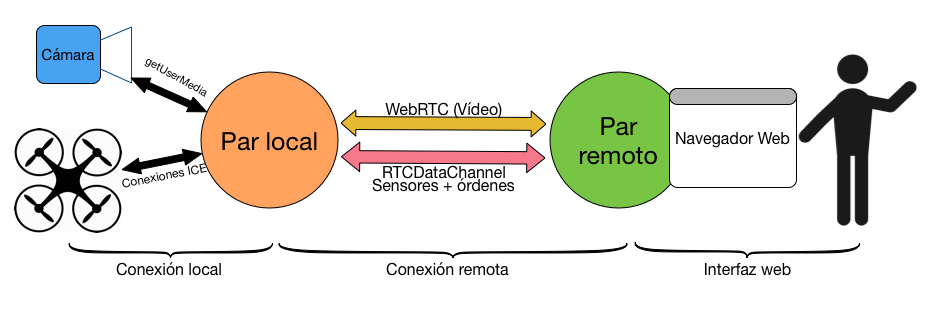
\includegraphics[width=1.1\textwidth]{img/esquema_general}
\end{figure}
\end{center}
\end{hslide}



%%--------------------------------------------------------------

\begin{hslide}
\slsubsect{Flujo de llamadas}
\begin{center}
\begin{figure}
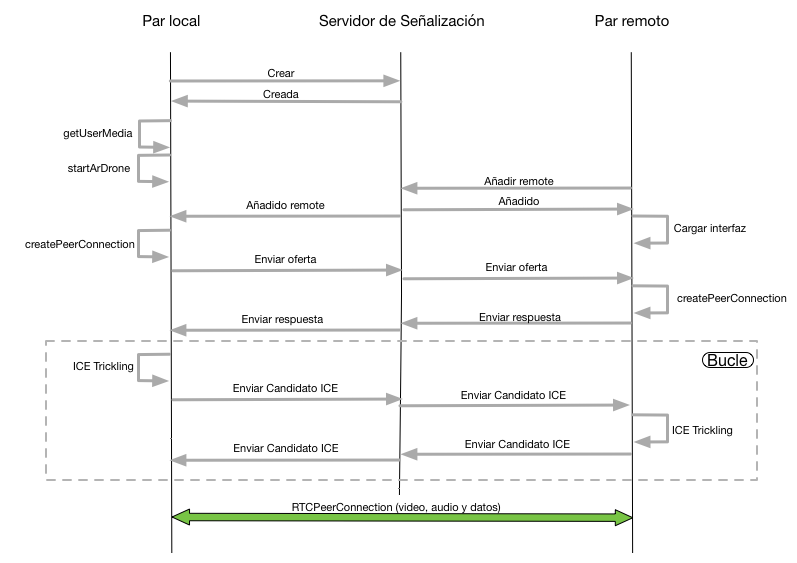
\includegraphics[width=0.8\textwidth]{img/diagrama_general}
\end{figure}
\end{center}
\end{hslide}

%%--------------------------------------------------------------

\begin{hslide}
\slsubsect{CONEXIÓN LOCAL}
\begin{minipage}[t]{0.6\textwidth}
\begin{itemize}
\item Esta conexión se divide en dos a su vez:
\begin{itemize}
\item \textbf{ArDroneServer y WebSockets:} Conexión entre el navegador y el drone. Cuatro interfaces ICE.
\item \textbf{getUserMedia:} El navegador accede a la cámara utilizando la API de WebRTC.
\end{itemize}
\end{itemize}

\end{minipage}
\begin{minipage}[t]{0.6\textwidth}
\begin{center}
\begin{figure}
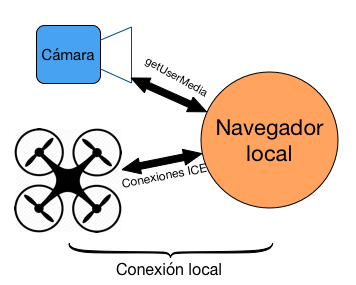
\includegraphics[width=0.9\textwidth]{img/conexionlocal}
\end{figure}
\end{center}
\end{minipage}
\end{hslide}


%%--------------------------------------------------------------

\begin{hslide}
\slsubsect{ArDroneServer y WebSockets}
\begin{itemize}
\item Para establecer la conexión se han activado los WebSockets de ICEJS en el archivo de configuración del servidor ArDroneServer.
\end{itemize}
\lstset{}
\begin{lstlisting}
 Ice.Plugin.IceWS=IceWS:createIceWS
\end{lstlisting}
\begin{itemize}
\item En el lado cliente la conexión mediante promesas de JavaScript.
\end{itemize}

\begin{center}
\begin{figure}
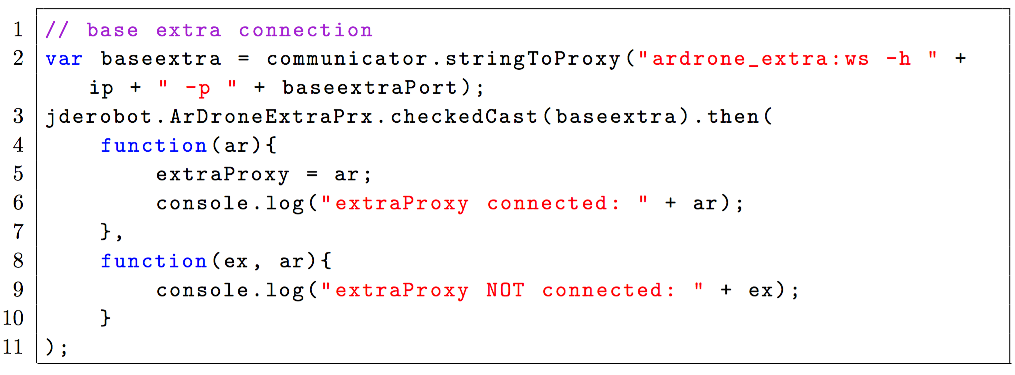
\includegraphics[width=0.9\textwidth]{img/promiseconexionlocal}
\end{figure}
\end{center}
\end{hslide}

%%--------------------------------------------------------------

\begin{hslide}
\slsubsect{getUserMedia}
\begin{center}
\begin{figure}
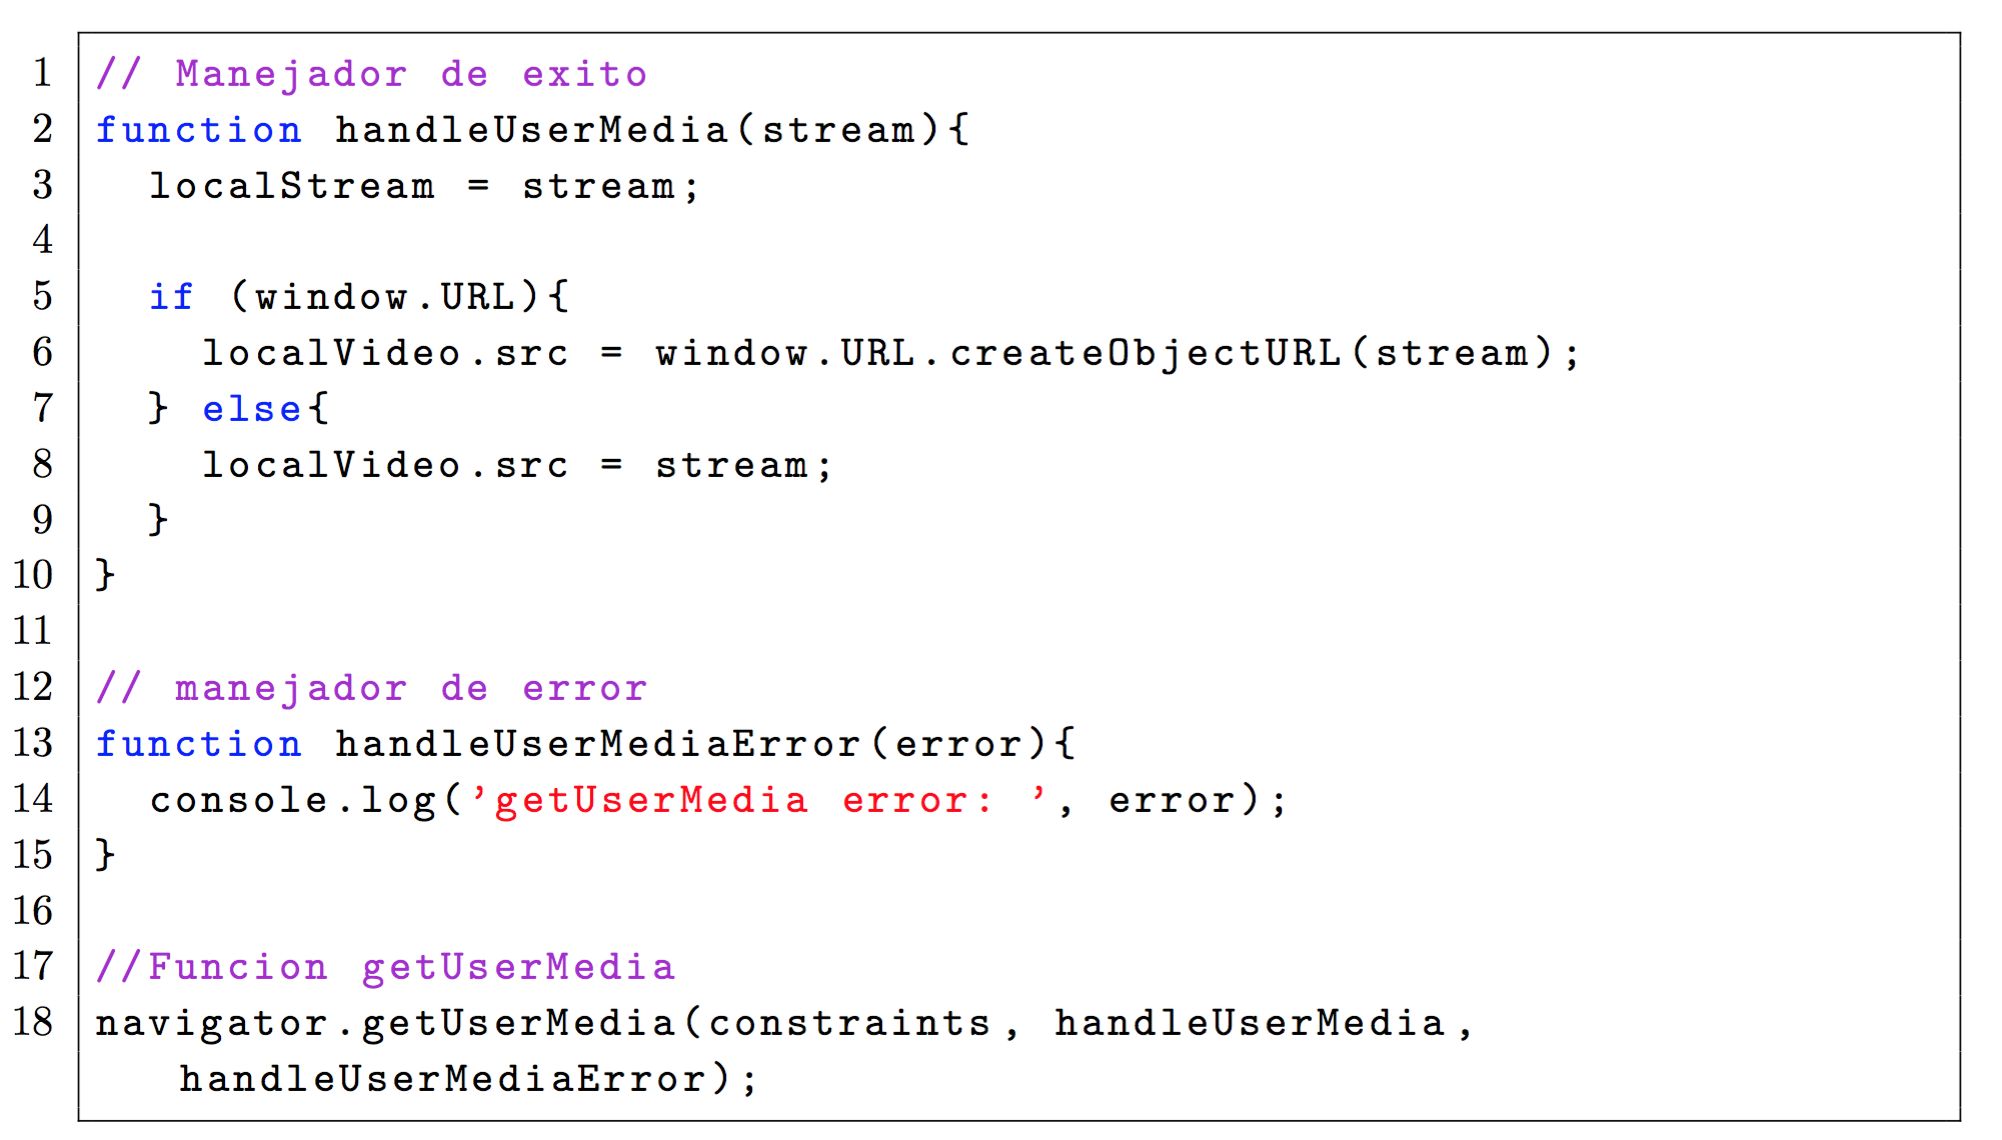
\includegraphics[width=1.1\textwidth]{img/getusermedia}
\end{figure}
\end{center}
\end{hslide}


%%--------------------------------------------------------------

\begin{hslide}
\slsubsect{CONEXIÓN ENTRE NAVEGADORES}
\begin{minipage}[t]{0.6\textwidth}
\begin{itemize}
\item Servidor de señalización para: Descubrimiento de pares e intercambio de SDP.
\item Transferir el flujo audiovisual de la cámara.
\item Intercambio de datos: sensores, órdenes.
\end{itemize}

\end{minipage}
\begin{minipage}[t]{0.6\textwidth}
\begin{center}
\begin{figure}
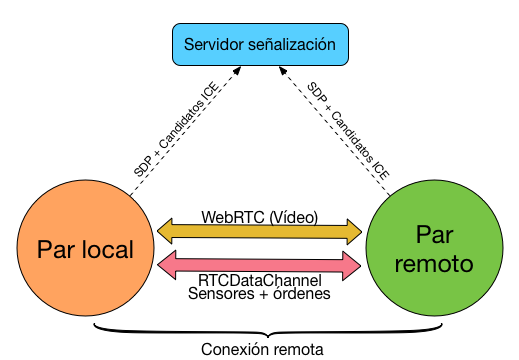
\includegraphics[width=0.9\textwidth]{img/conexionremota}
\end{figure}
\end{center}
\end{minipage}

\end{hslide}


%%--------------------------------------------------------------

\begin{hslide}
\slsubsect{Servidor de señalización}
\begin{itemize}
\item Escrito en Node.js
\item Intercambio de paquetes entre los pares con los descriptores de sesión y los candidatos ICE.
\item Librería \emph{Socket.io} para el intercambio de paquetes a través de \emph{WebSockets} entre los navegadores.
\item Desarrollado para satisfacer la arquitectura JSEP.
\end{itemize}
\end{hslide}

%%--------------------------------------------------------------

\begin{hslide}
\slsubsect{Transmisión de vídeo con RTCPeerConnection}
\begin{itemize}
\item Esta conexión se establece con la API \emph{RTCPeerConnection} de WebRTC.
\end{itemize}
\lstset{}
\begin{lstlisting}
var PC=new RTCPeerConnection(ICE_config,pc_constraints);
\end{lstlisting}

\begin{itemize}
\item El flujo obtenido con \emph{getUserMedia} se envía desde el par local al remoto a través de esta conexión.
\end{itemize}
\lstset{}
\begin{lstlisting}
 PC.addStream(localStream);
\end{lstlisting}
\end{hslide}

%%--------------------------------------------------------------

\begin{hslide}
\slsubsect{Transmisión de datos con RTCDataChannel}
\begin{itemize}
\item \emph{RTCDataChannel} de WebRTC permite transferir cualquier tipo de dato a través de \emph{RTCPeerConnection}.
\end{itemize}
\lstset{}
\begin{lstlisting}
DC=PC.createDataChannel("droneDataChannel",{ordered:false});
\end{lstlisting}

\begin{itemize}
\item Transfiere desde el navegador local al navegador remoto los datos de los sensores del drone.
\item Desde el par remoto al par local se transfieren las órdenes de movimiento dadas por el usuario final.
\end{itemize}
\end{hslide}


%%--------------------------------------------------------------

\begin{hslide}
\slsubsect{INTERFAZ WEB DE USUARIO EN CLIENTE REMOTO}
\begin{center}
\begin{figure}
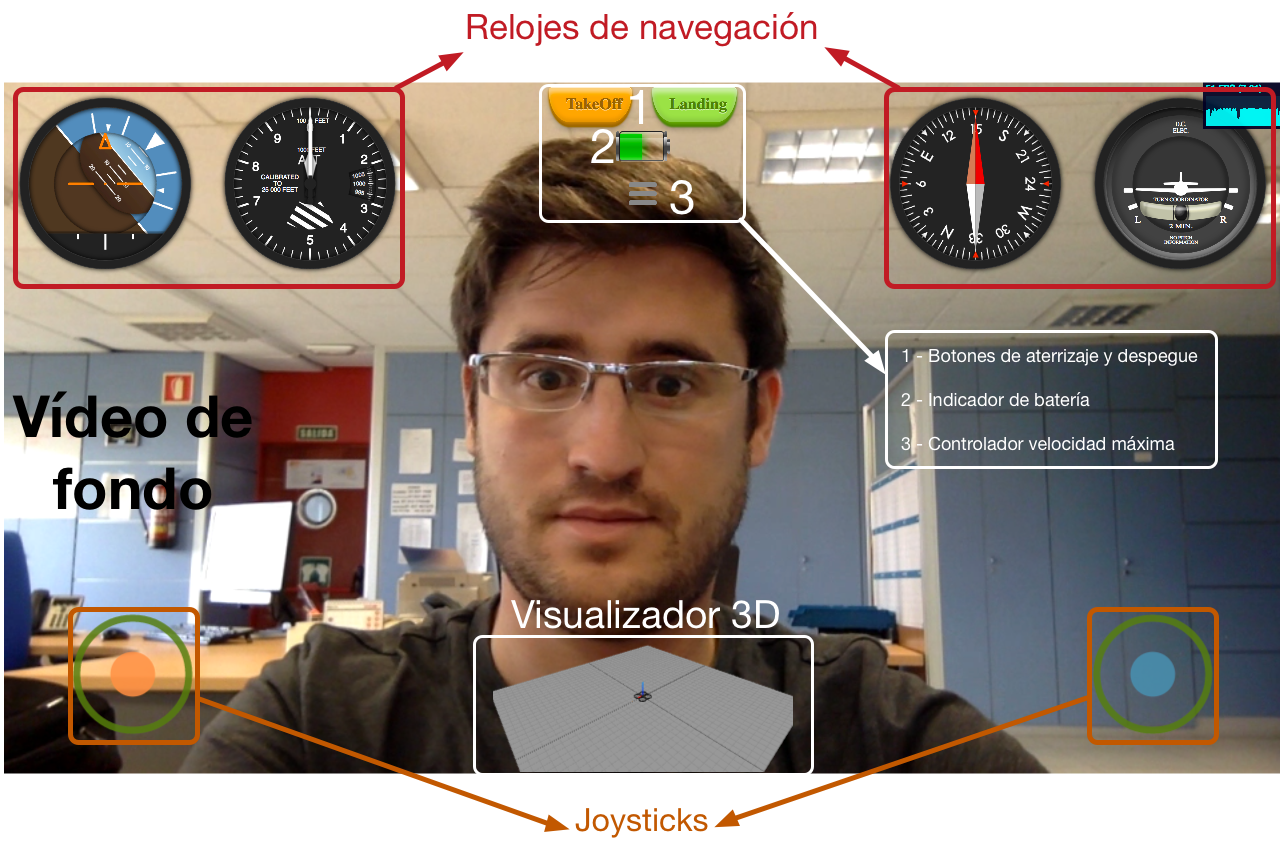
\includegraphics[width=0.9\textwidth]{img/interfazweb}
\end{figure}
\end{center}
\end{hslide}

%%--------------------------------------------------------------

\begin{hslide}
\slsect{Experimentos}
\slsubsect{Experimento con el simulador Gazebo}
\begin{itemize}
\item Realización de los experimentos de forma progresiva que validen que se han cumplido los objetivos.
\item Primero pruebas en el entorno virtual Gazebo para depurar el código.
\end{itemize}

\begin{minipage}[t]{0.3\textwidth}
\includegraphics[width=\textwidth]{img/experimentogazebo}
\end{minipage}
\begin{minipage}[t]{0.7\textwidth}
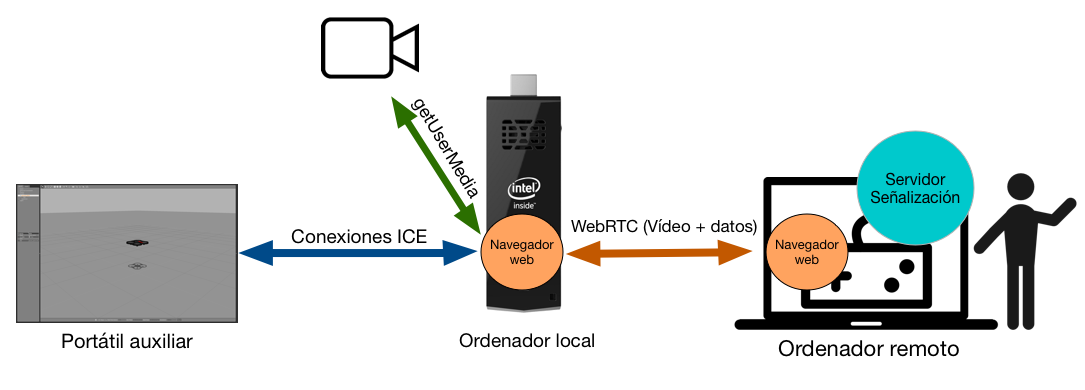
\includegraphics[width=\textwidth]{img/experimento1}
\end{minipage}
\end{hslide}

%%--------------------------------------------------------------

\begin{hslide}
\slsubsect{Experimento con drone real}
\begin{itemize}
\item Siguiente paso con el drone real sin poner a bordo el \emph{Computer Stick}.
\end{itemize}

\begin{minipage}[t]{0.3\textwidth}
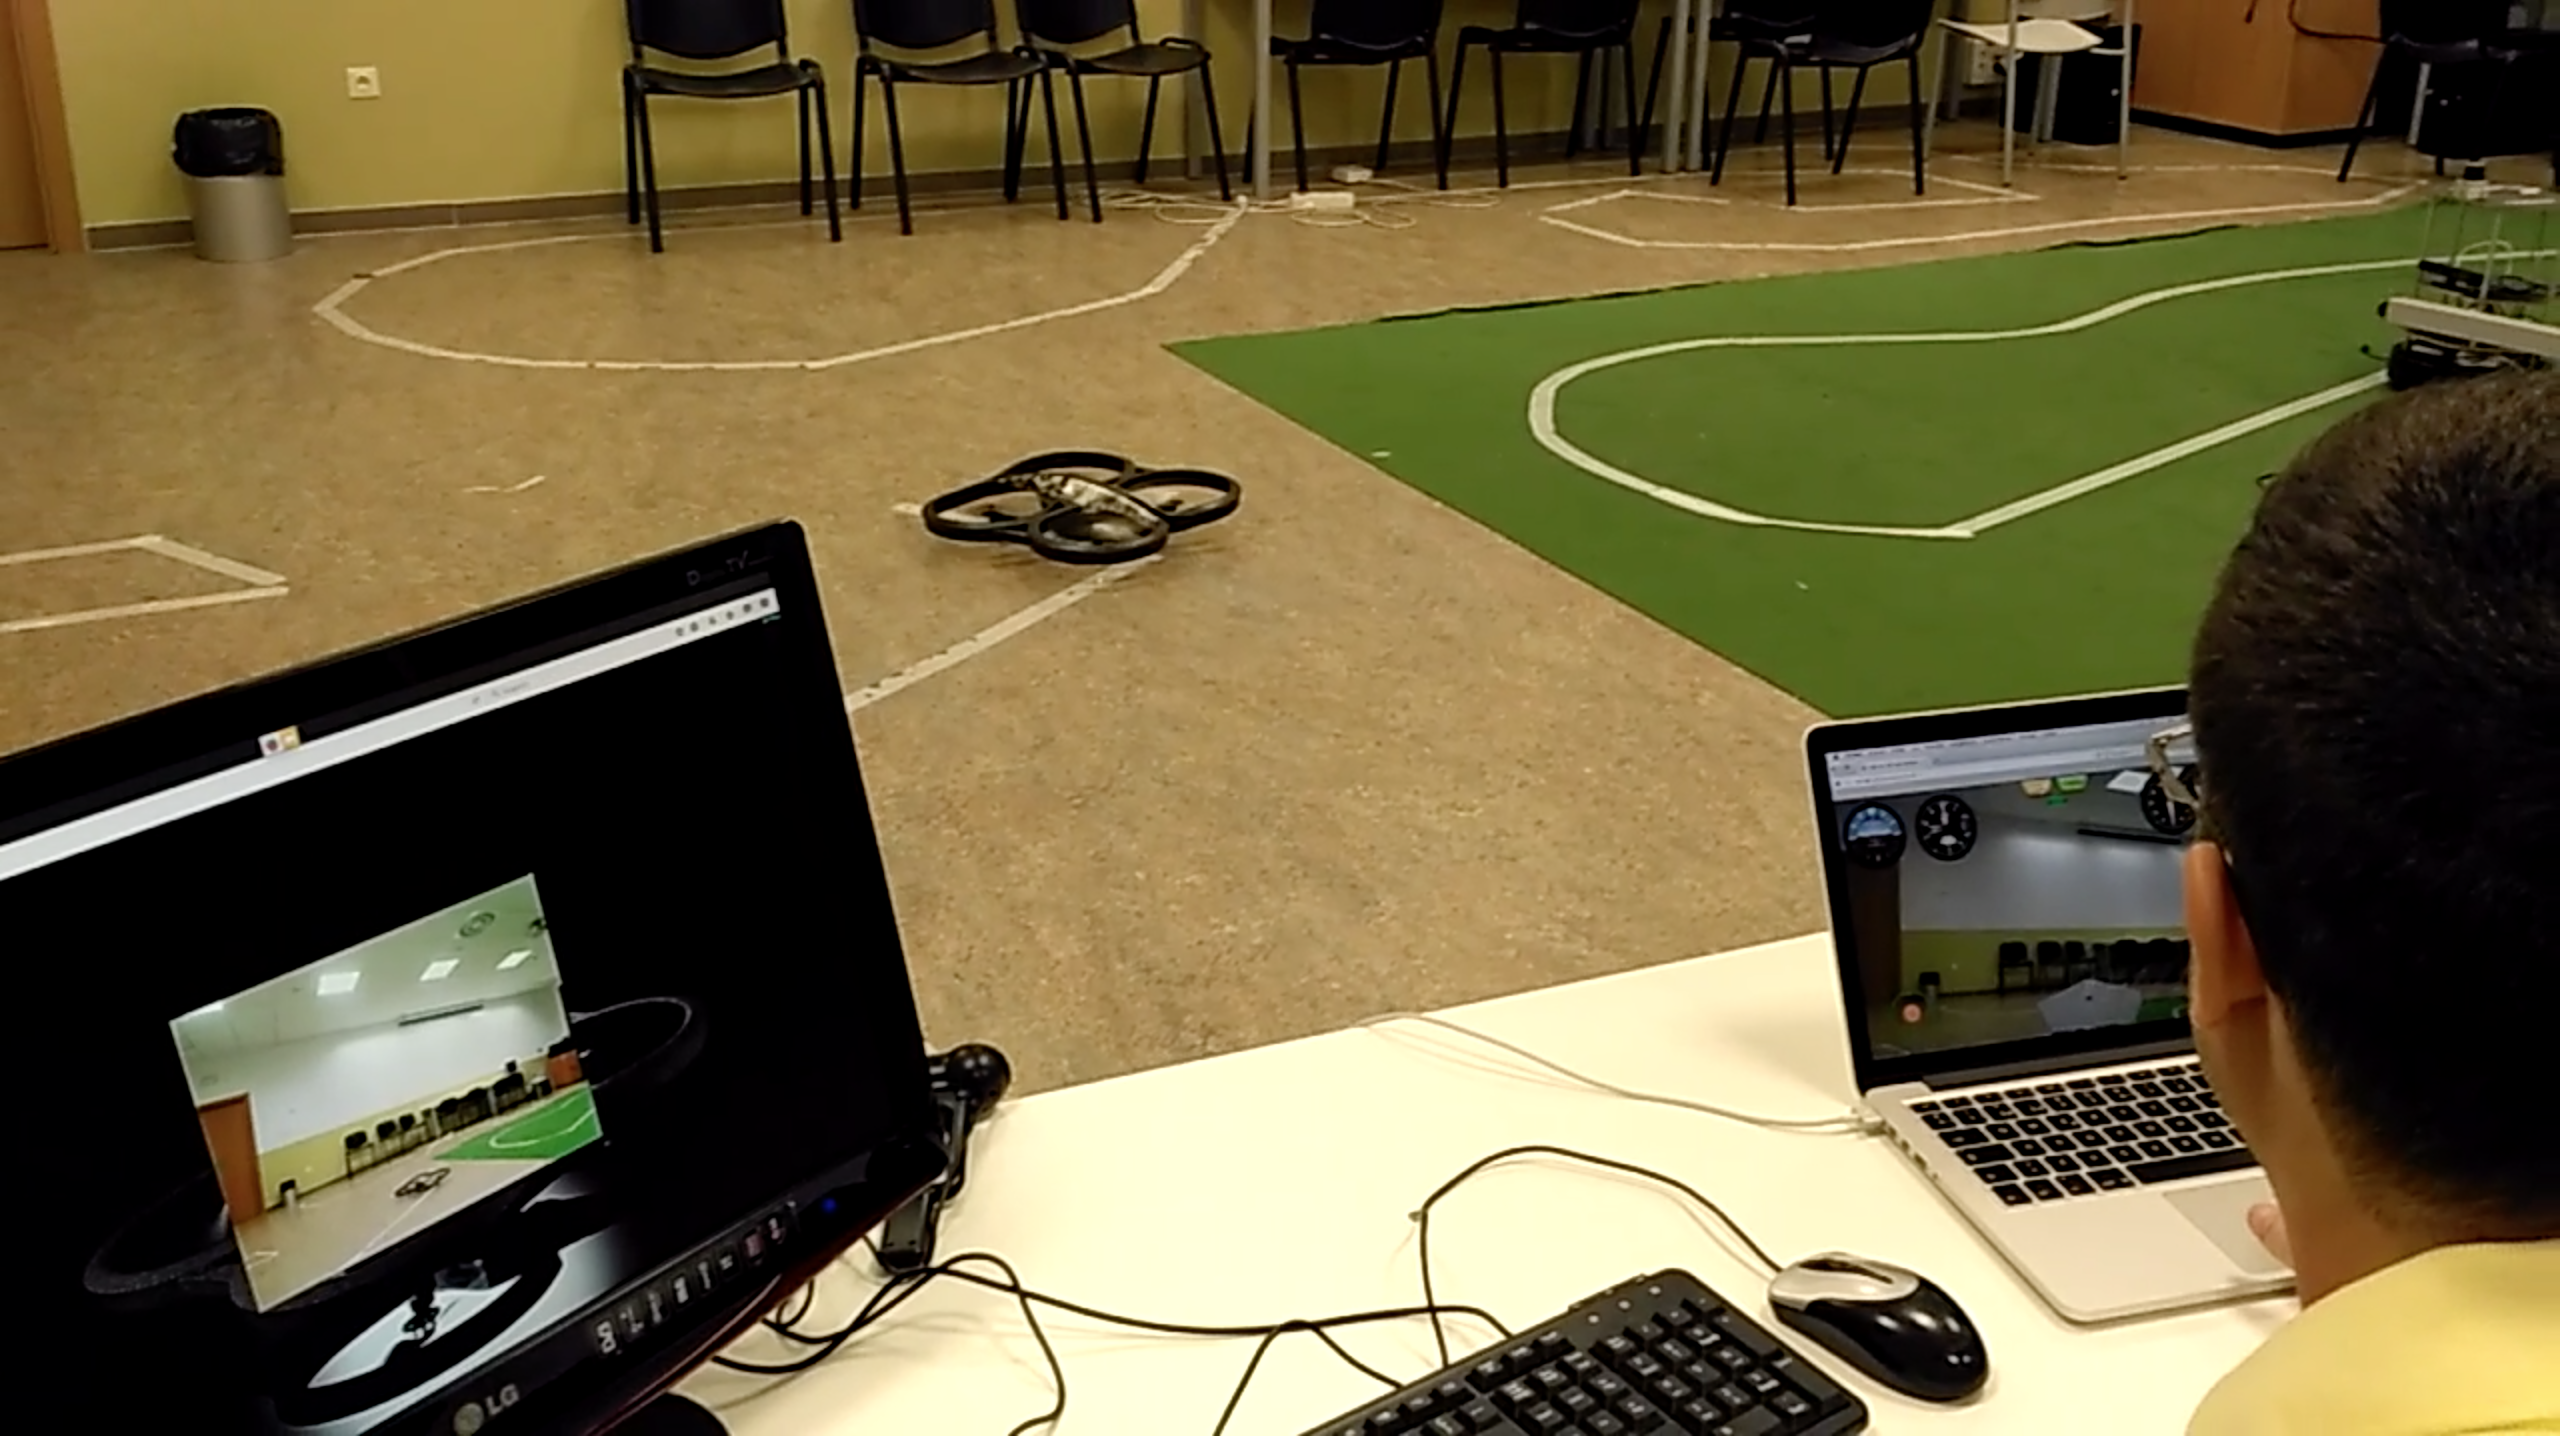
\includegraphics[width=\textwidth]{img/experimentodronereal1}
\end{minipage}
\begin{minipage}[t]{0.7\textwidth}
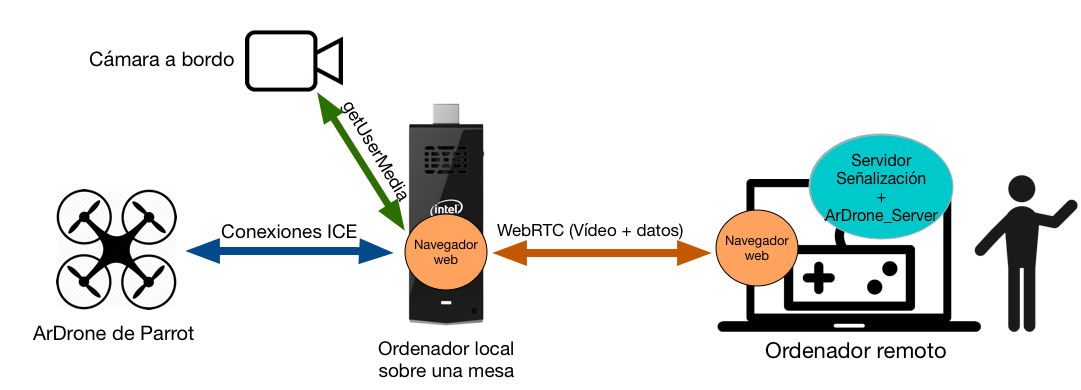
\includegraphics[width=\textwidth]{img/esquema_experimento2}
\end{minipage}

\end{hslide}

%%--------------------------------------------------------------

\begin{hslide}
\slsubsect{Experimento todo en drone real}
\begin{itemize}
\item \emph{Computer Stick} a bordo del drone.
\item El resultado del experimento es fallido: no puede con el peso.
\item El peso de la cámara, el \emph{Computer Stick} y la pila para alimentarlo supera la carga de peso máxima permitida por este drone.
\end{itemize}
\end{hslide}

%%--------------------------------------------------------------

\begin{hslide}
\begin{minipage}[t]{0.4\textwidth}
\includegraphics[width=\textwidth]{img/elementos_abordo}
\end{minipage}
\begin{minipage}[t]{0.6\textwidth}
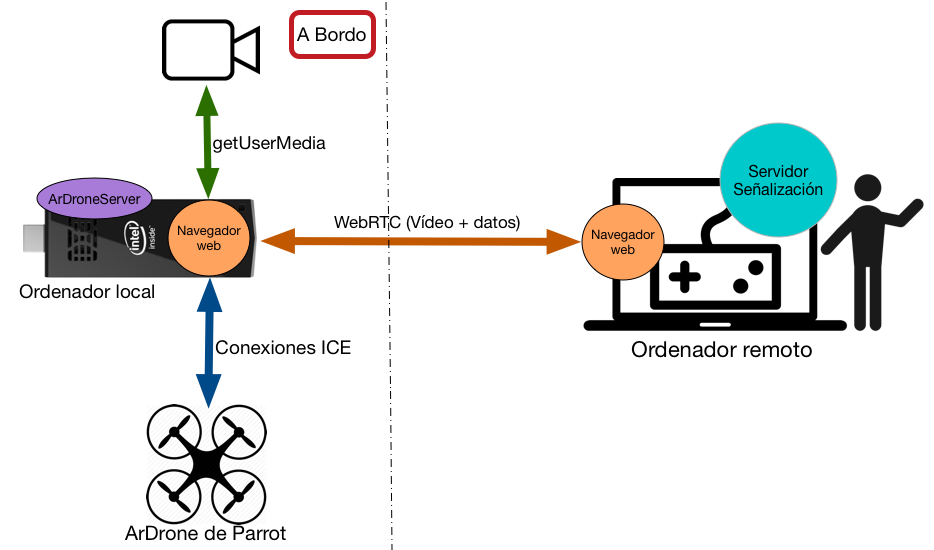
\includegraphics[width=\textwidth]{img/esquema_experimento_abordo}
\end{minipage}

\begin{minipage}[t]{0.5\textwidth}
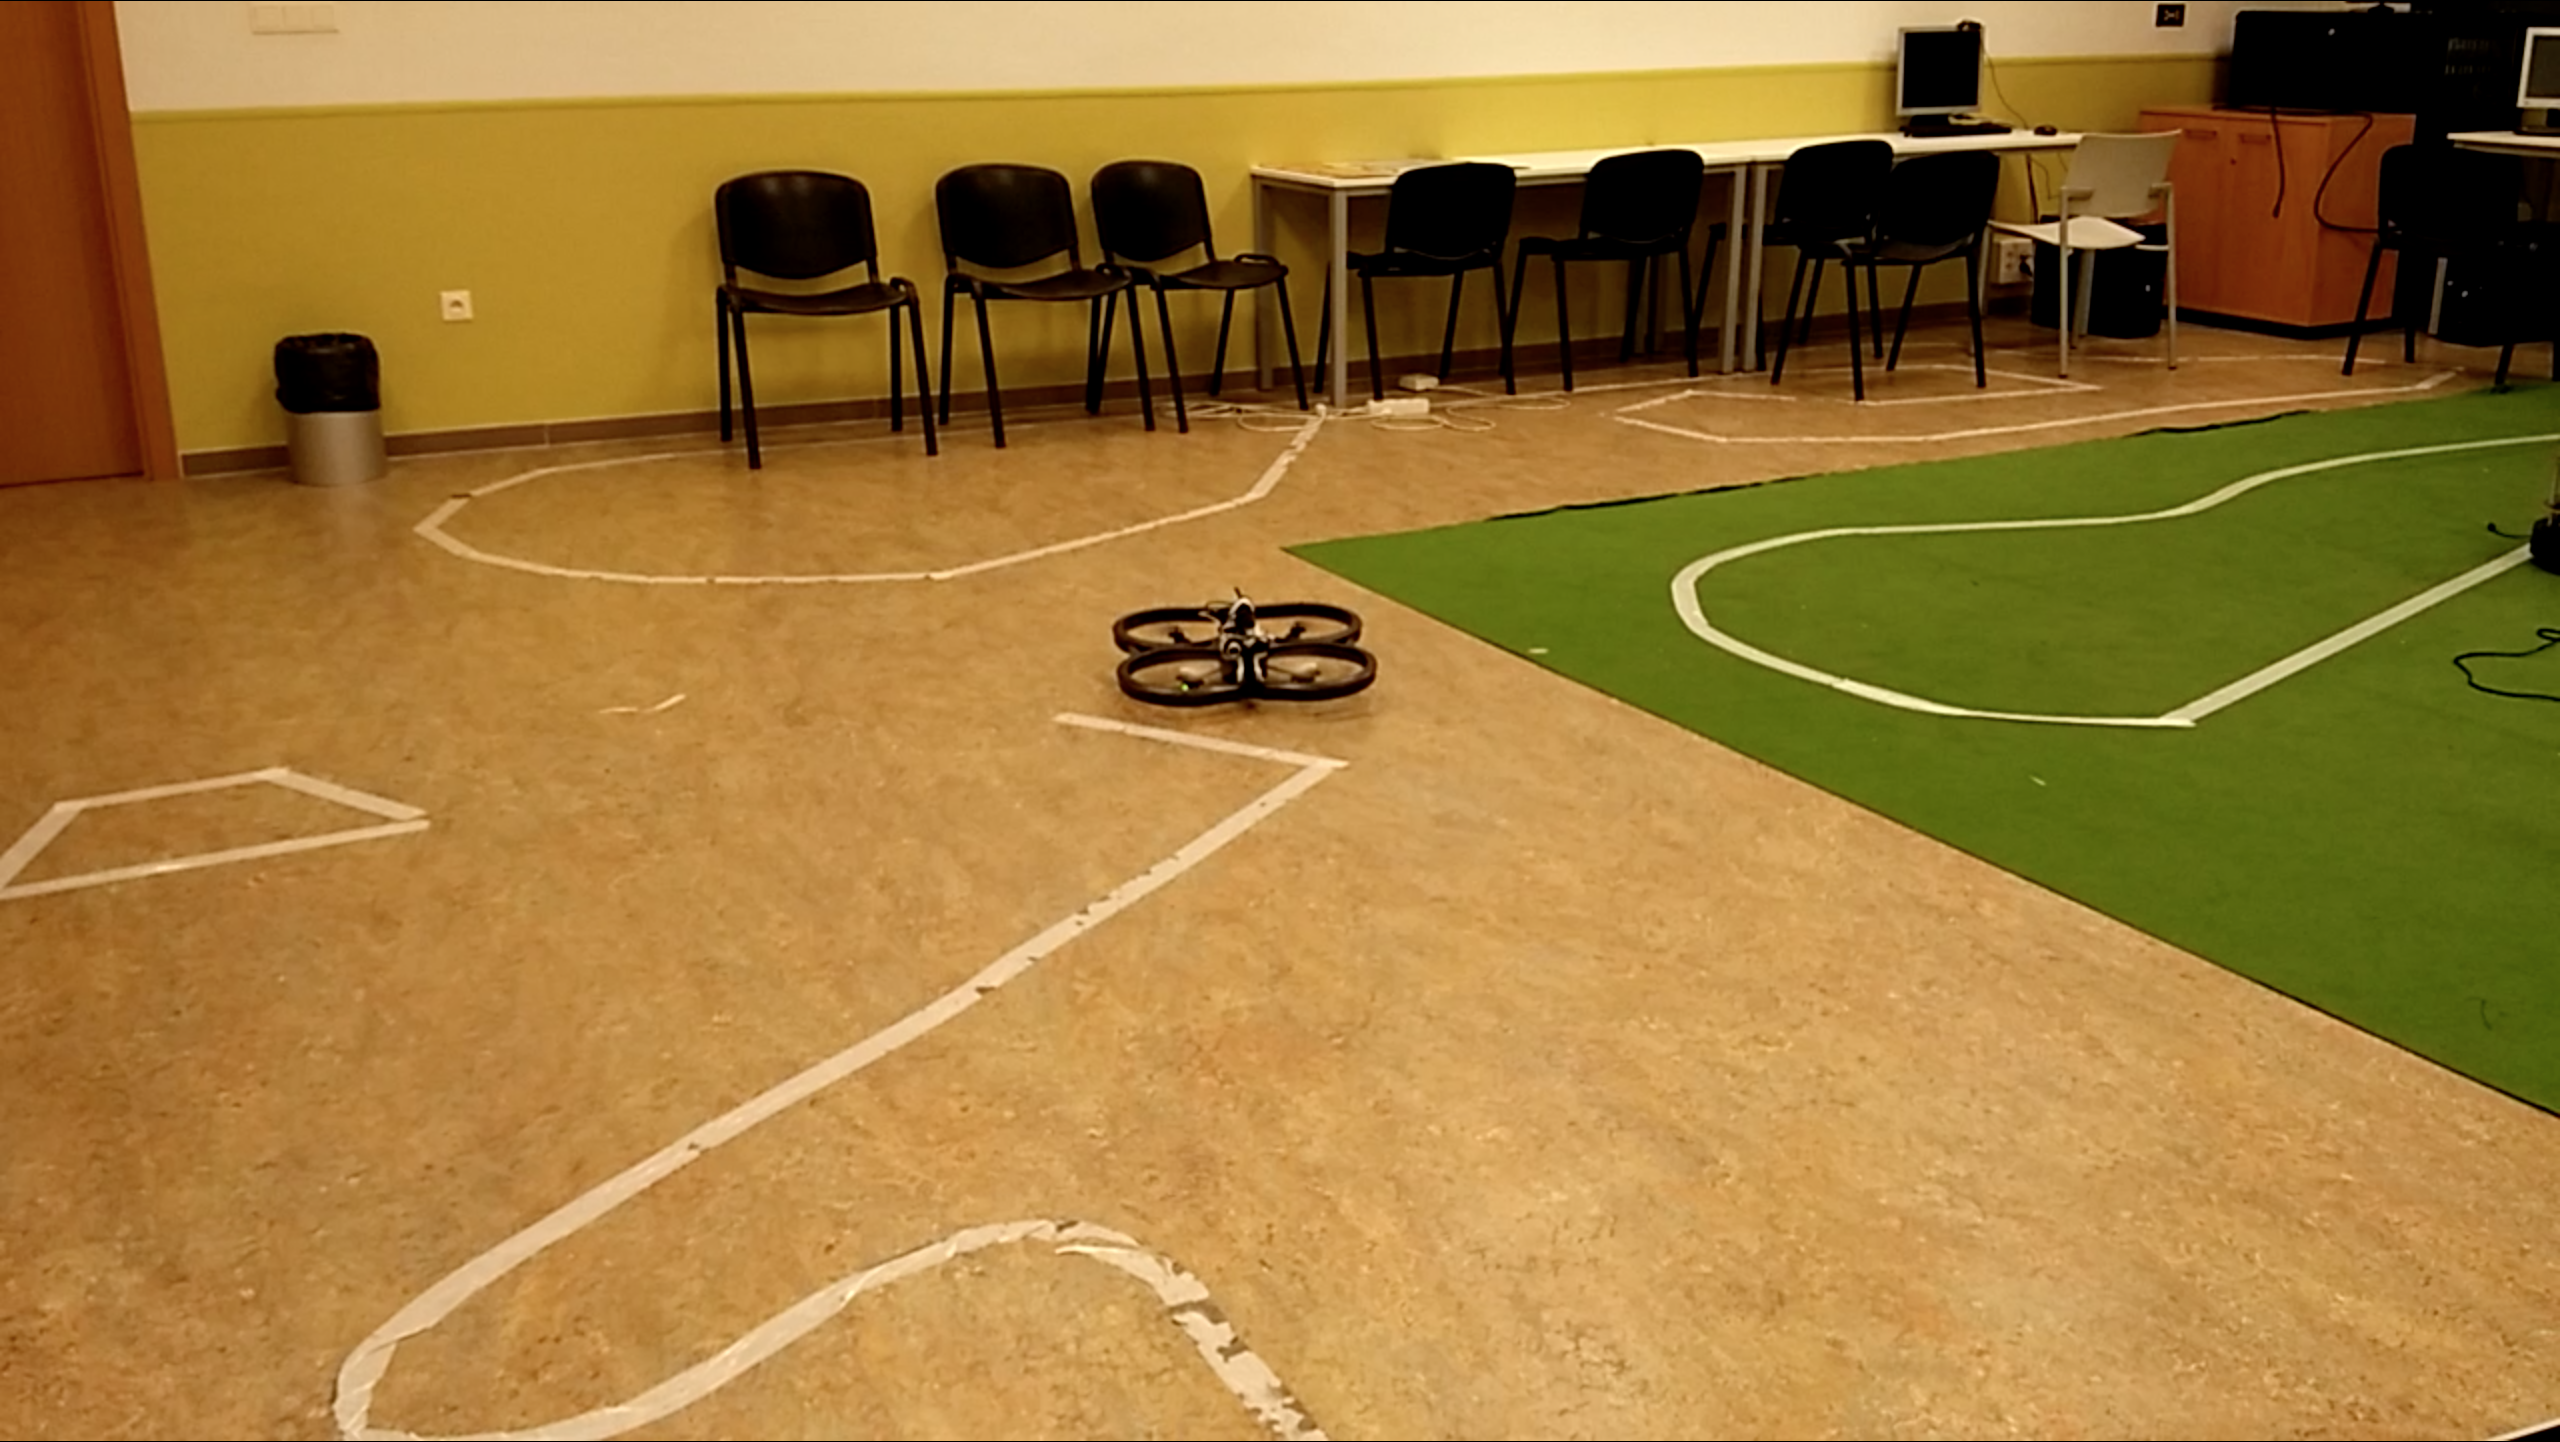
\includegraphics[width=\textwidth]{img/experimento_abordo}
\end{minipage}
\begin{minipage}[t]{0.5\textwidth}
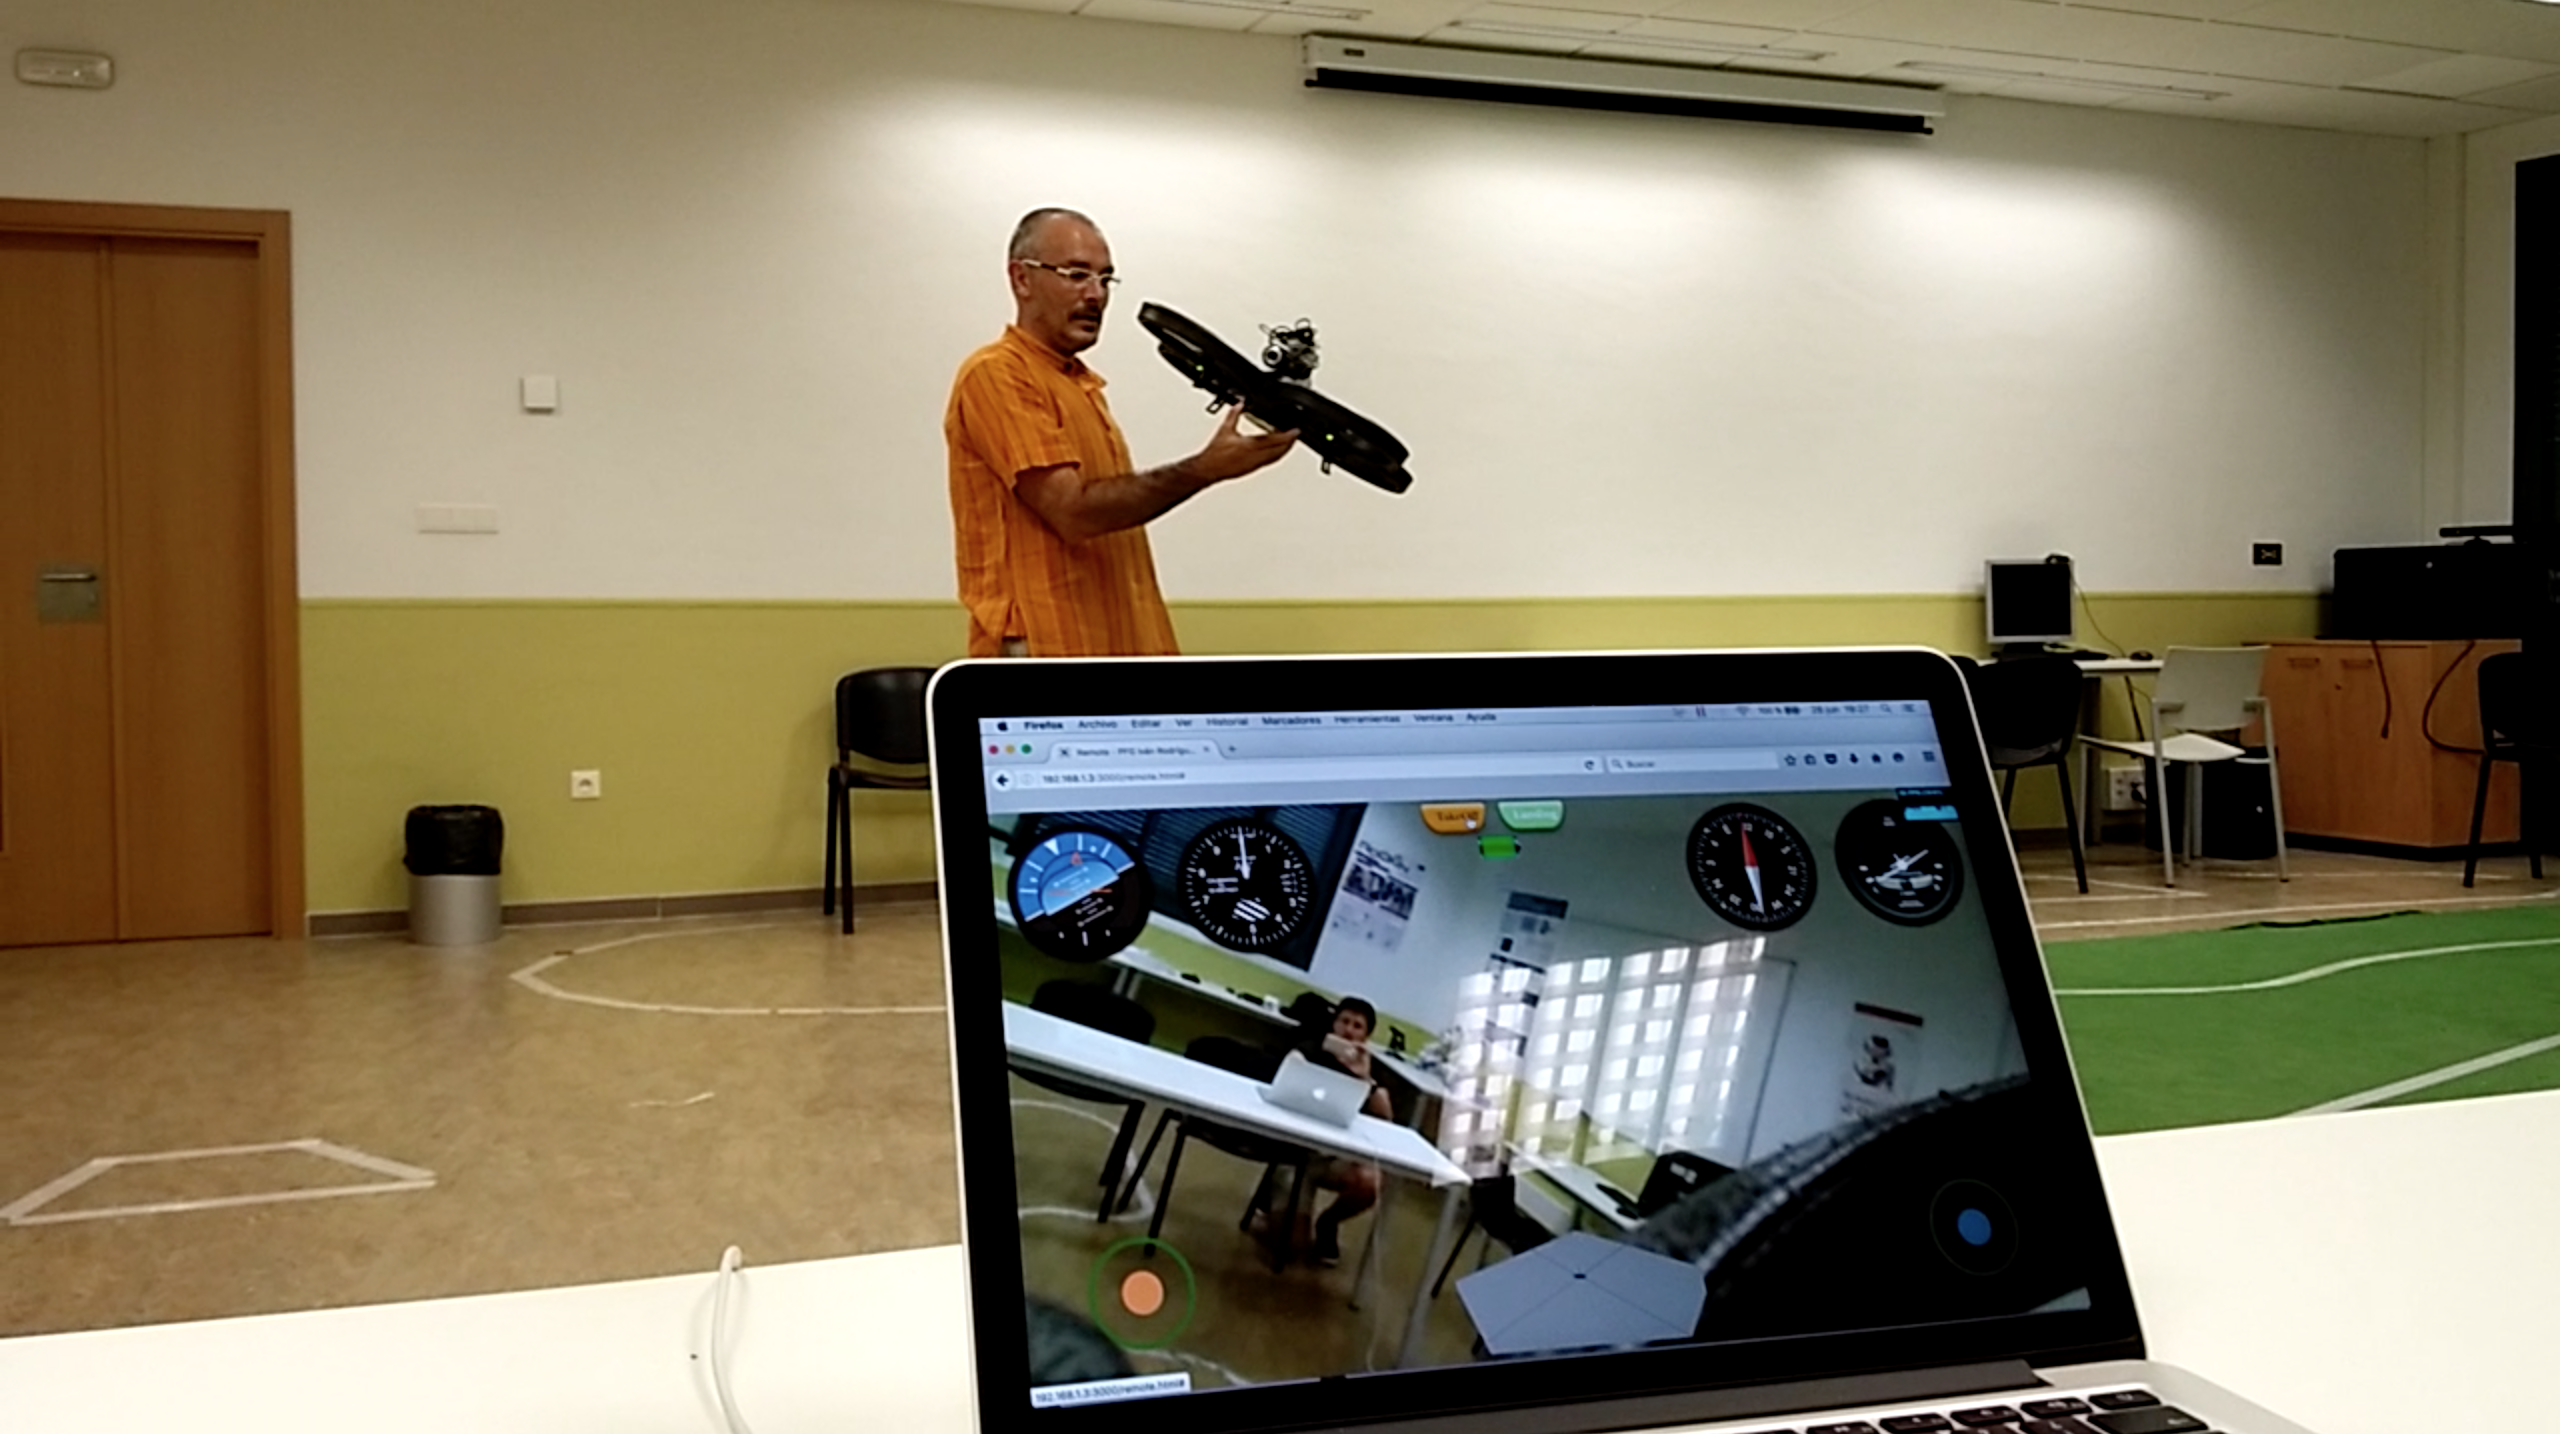
\includegraphics[width=\textwidth]{img/pruebas_experimento_abordo}
\end{minipage}
\end{hslide}

%%--------------------------------------------------------------

\begin{hslide}
\slsubsect{Experimentos con multidispositivo}
\begin{itemize}
\item Dos experimentos con configuraciones diferentes.
\end{itemize}
\begin{minipage}[t]{0.4\textwidth}
\includegraphics[width=\textwidth]{img/experimentodronemultidispositivo1}
\end{minipage}
\begin{minipage}[t]{0.6\textwidth}
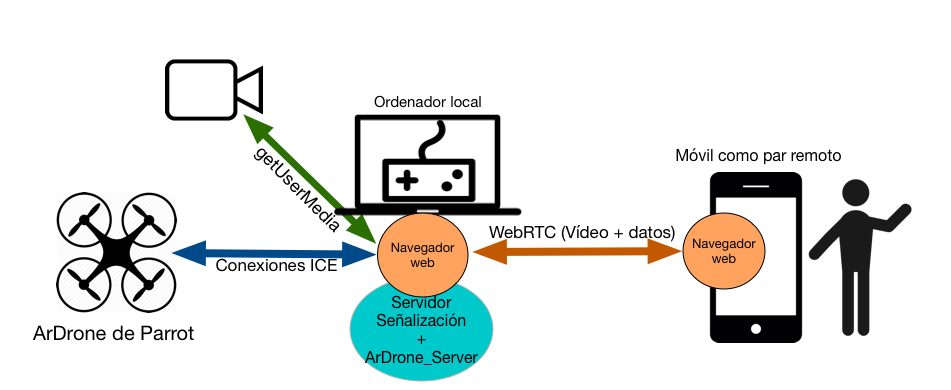
\includegraphics[width=\textwidth]{img/esquema_experimento_multidispositivo_1}
\end{minipage}

\begin{minipage}[t]{0.4\textwidth}
\includegraphics[width=\textwidth]{img/experimentodronemultidispositivo2}
\end{minipage}
\begin{minipage}[t]{0.6\textwidth}
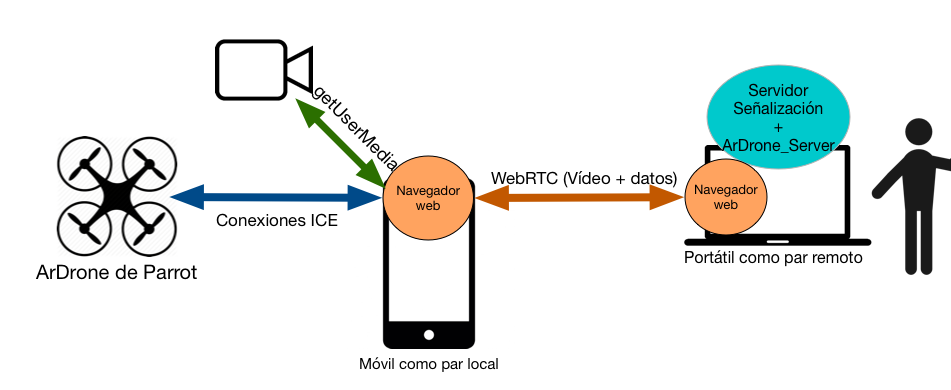
\includegraphics[width=\textwidth]{img/experimento_multidispositivo2}
\end{minipage}

\end{hslide}

%%--------------------------------------------------------------

\begin{hslide}
\slsect{Conclusiones}
\begin{itemize}
\item \textbf{Objetivo cumplido}: capacidad de teleoperar el drone con tecnologías web de última generación y sin necesidad de servidores intermedios.
\item Conexiones en tiempo real
\item Interfaz web amigable e intuitiva.
\item Multitplataforma y multidispositivo.
\item Todo lo desarrollado ha quedado validado con los experimentos.
\end{itemize}
\vspace{0.5cm}
Líneas futuras:
\begin{itemize}
\item Teleoperar el drone con coordenadas que permitan tener autonomía.
\item Integración en el repositorio oficial de JdeRobot.
\end{itemize}
\end{hslide}

%%--------------------------------------------------------------

\begin{hslide}
\slsect{Enlaces}
\begin{itemize}
\item Mediawiki: \url{http://jderobot.org/Irodmar-tfg}
\item Repositorio: 
\begin{itemize}
\item \url{https://github.com/RoboticsURJC-students/2015-tfg-irodmar}
\end{itemize}
\end{itemize}
\end{hslide}

\end{document}